\documentclass[aps,prx,reprint,superscriptaddress,footnote, twocolumn,notitlepage]{revtex4-2}
%\usepackage[T1]{fontenc}
%\usepackage[utf8x]{inputenc}
%\usepackage[sc,osf]{mathpazo}\linespread{1.05}
\usepackage{amsmath, amsthm, amssymb,amsfonts,mathbbol,amstext}
\usepackage{braket}
\usepackage{pifont}
\usepackage{graphicx}
\usepackage{dcolumn}
\usepackage{bm}
\usepackage{bbm}
\usepackage{hyperref}
\usepackage{mathtools}
\usepackage{comment}
\usepackage{color}
\usepackage{multirow}
\usepackage{diagbox}
\usepackage{float}
\usepackage{xcolor}
\usepackage{makecell}
\usepackage[normalem]{ulem}
\usepackage{soul}
\usepackage{tikz}
\newcommand{\yu}[1]{\textcolor{blue}{#1}}
\newcommand{\tom}[1]{\textcolor{green}{#1}}
\newcommand{\ko}[1]{\textcolor{orange}{#1}}
\newcommand{\ph}[1]{\textcolor{purple}{#1}}


\newcommand{\todoyu}[1]{\yu{$\heartsuit$ #1}}
\newcommand{\todotom}[1]{\tom{$\spadesuit$ #1}}
\newcommand{\todoko}[1]{\ko{$\diamondsuit$ #1}}
\newcommand{\todoph}[1]{\ph{$\clubsuit$ #1}}

% Language setting
% Replace `english' with e.g. `spanish' to change the document language
\usepackage[english]{babel}

% Set page size and margins
% Replace `letterpaper' with `a4paper' for UK/EU standard size
\usepackage[letterpaper,top=2cm,bottom=2cm,left=3cm,right=3cm,marginparwidth=1.75cm]{geometry}

% Useful packages
\usepackage{amsmath}
\usepackage{graphicx}
% \usepackage[colorlinks=true, allcolors=blue]{hyperref}

\begin{document}
\title{Look Mum No Hands: reachability in autonomous quantum systems \ko{(working title)}}


\author{Tomasz Andrzejewski}
\email{tomasz.andrzejewski@tuwien.ac.at}
\affiliation{Atominstitut, Technische Universit{\"a}t Wien, Stadionallee 2, 1020 Vienna, Austria}

\author{Yuri Minoguchi}
\affiliation{Atominstitut, Technische Universit{\"a}t Wien, Stadionallee 2, 1020 Vienna, Austria}


\author{Phila Rembold}
\affiliation{Atominstitut, Technische Universit{\"a}t Wien, Stadionallee 2, 1020 Vienna, Austria}

\author{Konrad Szyma\'nski}
\email{k.sz@quantumstat.es}
\affiliation{Research Center for Quantum Information, Slovenská Akadémia Vied, Dúbravská cesta 9, 84511 Bratislava, Slovakia}
\affiliation{Naturwissenschaftlich-Technische Fakultät, Universität Siegen, Walter-Flex-Straße 3, 57068 Siegen, Germany}


%\begin{abstract}
%Things to do (feel free to pick yr color):\\
%\todoko{Konrad}\\
%\todotom{Tomek}\\
%\todoyu{Yuri}\\
%\todoph{Phila}
%\end{abstract}


\maketitle
\section{Introduction}

Quantum control theory addresses how to steer quantum systems between states and turn abstract quantum processes into concrete control protocols~\cite{koch_quantum_2022,Glaser2015,weidner_energy_2025, ansel_introduction_2024}. The standard toolbox relies on time-varying fields, such as lasers and oscillating magnetic fields, translating to control Hamiltonians to navigate Hilbert space~\cite{theis_counteracting_2018, rodzinka_optimal_2024, Rembold2020}. By exploiting the complexity introduced through time dependence, these approaches provide bespoke control strategies. However, this flexibility comes at a price: time-varying controls are never perfect, introducing their own sources of noise, and dynamic control demands rapid modulation with high resolution, often requiring specialised experimental setups.
%This approach is powerful but has drawbacks: gate sequences accumulate noise, degrading fidelity exponentially with circuit depth, and dynamic control demands rapid modulation at significant speed and resolution.

% cite{schirmer_design_2018}\cite{meier_autonomous_2024} -- energetics of computation

Fortunately, time-varying fields are not the only option. An alternative is to design a time-independent Hamiltonian such that autonomous evolution carries the system from the initial to the target state. This approach requires only calibration ahead of time rather than continuous adjustment offering both simplicity and provable robustness~\cite{schirmer_design_2018, weidner_energy_2025}. Frameworks that provide such autonomous controls can be characterised and calibrated with Hamiltonian learning~\cite{kraft_bounded_2025}. Protocols for finding the appropriate time-independent Hamiltonian within a naturally achievable family, sometimes referred to as ``energy landscape shaping'', have been designed for spin chains~\cite{schirmer_design_2018}, optical lattices~\cite{weidner_energy_2025}, and abstract qubit networks~\cite{cieslinski_fastest_2023}. Other work shows that piecewise-constant time-dependent protocols can be translated directly into autonomous controls using auxiliary systems~\cite{mooney_time_2025I} without loosing information propagation speed~\cite{mooney_time_2025II}.
\begin{figure}
    \centering
    \includegraphics[width=0.9\linewidth]{fig/fig1.png}
 \caption{Schematic of reachability in Hilbert space. Given an initial state and a parametrized family of Hamiltonians $H = \sum_n \lambda_n H_n$, only a subset of states may be reachable via autonomous evolution. Colored trajectories represent orbits under different permissible Hamiltonians. The three criteria developed in this work are illustrated: \textbf{(a)} Spectral Criterion: States sharing the same eigenstate probabilities $p_i = |\langle \alpha_i | \phi \rangle|^2$ form invariant manifolds (depicted as a torus); the criterion optimizes over Hamiltonians to maximize the overlap $S = \sum_i \sqrt{p_i q_i}$ between initial and target spectral distributions. \textbf{(b)} Moment: Conservation of $\langle H \rangle$ and $\langle H^2 \rangle$ defines a quadratic form $M(\gamma)$; if $M(\gamma)$ is positive definite for some $\gamma$, unreachability is certified without optimization. \textbf{(c)} Krylov: The target must lie within the Krylov subspace $\mathcal{K} = \mathrm{span}\{|\phi\rangle, H|\phi\rangle, H^2|\phi\rangle, \ldots\}$; the criterion optimizes the projection $K = \|\Pi_{\mathcal{K}}|\psi\rangle\|$ over the Hamiltonian family.}%{Depending on the allowed initial states and family of Hamiltonians, it is possible that only a portion of Hilbert space is reachable. Pictured is a symbolic sketch of orbits corresponding to various Hamiltonians, together with the symbolic meaning of the three criteria forming the result of this paper: a) for a given Hamiltonian a set of states with the same spectral properties as the input states forms a torus, the spectral criterion optimizes the Hamiltonians, and subsequently tori, to find the one closest to the target state; b) the moment criterion makes use of a quadratic form, which, if positive, ascertains that a given target state is unreachable for any hamiltonian in the given family; c) the Krylov criterion calculates the Krylov subspace for any given Hamiltonian, the overlap of the subspace with the target state is optimized. }%{Dependent on the set of Hamiltonians, only part of the Hilbert space is reachable. The portion depends on the given set.}
    \label{fig:hilbert}
\end{figure}

Beyond certain practical advantages, the role of autonomous evolution is more foundational. For example, Meier et al.~\cite{meier_autonomous_2024} constructed an autonomous quantum processing unit (a machine requiring no input after initial preparation
%, analogous to the billiard-ball model of Fredkin and Toffoli \cite{Fredkin2002}
) from which fundamental thermodynamic limits of quantum computation can be derived. Here, autonomous evolution is crucial to keep classical controls from obscuring the resource accounting. Similarly, autonomous quantum cellular automata can be used to construct passive, self-correcting quantum memory~\cite{dunnweber_quantum_2026}. 
%The assumption of autonomous evolution also simplifies verification of the Hamiltonian weights, as compared to general time-varying one~\cite{kraft_bounded_2025}. 
Considering the autonomous dynamics of locally interacting qubit grids, sampling transition probabilities generated by autonomous controls are believed to be classically intractable~\cite{quek2025quantumadvantagerandomgeometricallytwolocal, park2023hardnessquantumspindynamics}. This mirrors the computational hardness underlying boson sampling~\cite{aaronson_computational_2010} connecting complexity-theoretic insights of autonomous controls to quantum advantage considerations.
%On the other hand, it is computationally difficult to sample transition probabilities emerging from autonomous evolution in qubit grids \cite{quek2025quantumadvantagerandomgeometricallytwolocal, park2023hardnessquantumspindynamics}, in much the same way as for boson sampling problem \cite{aaronson_computational_2010}. 
However, computational power is not the same thing as a guarantee of full Hilbert space exploration \todoko{(somehow play with the `tiny corner of hilbert space' idea)}, and restricted Hamiltonian families may still have limited reachability.

A natural question is how expressive autonomous evolution can be. Restricted Hamiltonian families may possess conserved quantities that limit reachability even without obvious symmetry structure; for instance, qubit odd-body Hamiltonians preserve certain values that even-body Hamiltonians do not~\cite{wyderka_constraints_2018}, rendering some sectors of the Hilbert space unreachable from initial product states.

Here we study these limits systematically. We introduce model systems in Sec.~\ref{sec:systems}, including abstract qudits with general interactions and qubit grids with geometrically constrained couplings. In Sec.~\ref{sec:crit} we develop three criteria for determining reachability: two analytical conditions that can certify unreachability, and one based on numerical optimization (see Fig.~\ref{fig:hilbert}). In Sec.~\ref{sec:results} we study how the fraction of reachable states depends on the Hilbert space dimension and the number of available Hamiltonian generators.


\section{Analyzed systems}\label{sec:systems}
\subsection{Abstract qudit Hamiltonians}
\label{sec:canonical}

The canonical basis provides a complete orthogonal basis for $d\times d$ Hermitian matrices. Any $d$-dimensional Hilbert space is spanned by its basis operators:
\begin{equation}
\begin{aligned}
X_{jk} &= |j\rangle\langle k| + |k\rangle\langle j| \quad (j < k), \\
Y_{jk} &= -i|j\rangle\langle k| + i|k\rangle\langle j| \quad (j < k), \\
Z_j &= |j\rangle\langle j| - |j+1\rangle\langle j+1| \quad (j = 0, \ldots, d-2), \\
I &= \mathbb{1}_d,
\end{aligned}
\label{eq:canonical_basis}
\end{equation}
where indices run over $j, k \in \{0, \ldots, d-1\}$. %This gives $d^2$ operators total: $d(d-1)/2$ operators each for $X$ and $Y$ types, $(d-1)$ operators of $Z$ type, and the identity. 
The qudit states $\ket{j}$ can be interpreted as a particle localised at the discrete site $j$, and the operators $X_{jk}, Y_{jk}$ describe hopping between sites. The full basis provides an abstract reference for comparison with more limited families (next section).

\subsection{Qubit grids with limited interaction} \label{sec:geo2}

We also test our criteria on qubit grids with geometrically local interactions, relevant for quantum computing hardware. Consider $n = L_x \times L_y$ qubits arranged on a rectangular lattice of length $L_x$ and width $L_y$. The Hamiltonian family $\mathcal{P}_2$ consists of all 1-local and nearest-neighbor 2-local Pauli terms:

\begin{widetext}
\begin{equation}
H(\boldsymbol{\lambda}) = \sum_{i=1}^{n} \sum_{\alpha \in \{X,Y,Z\}} \lambda_{i,\alpha} \sigma_\alpha^{(i)} + \sum_{\langle i,j \rangle} \sum_{\alpha,\beta \in \{X,Y,Z\}} \lambda_{ij,\alpha\beta} \, \sigma_\alpha^{(i)} \sigma_\beta^{(j)},
\label{eq:geo2local}
\end{equation}
\end{widetext}
where $\sigma_\alpha^{(i)}$ denotes a Pauli matrix acting on site $i$, the sum $\langle i,j \rangle$ runs over nearest-neighbor pairs, and each edge can support any of the nine interaction types ($\sigma_X \sigma_Y$, \ldots, $\sigma_Z \sigma_Z$). The total number of generators is $3n + 9(2L_x L_y - L_x - L_y)$: three single-site terms per qubit plus nine two-body terms per edge.

Note that subfamilies of $\mathcal{P}_2$ may have additional structure. The transverse-field Ising Hamiltonian $H = -J \sum_{\langle i,j \rangle} \sigma_Z^{(i)} \sigma_Z^{(j)} - h \sum_i \sigma_X^{(i)}$ is a restricted subfamily using only $\sigma_Z \sigma_Z$ and $\sigma_X$ terms. Interactions of the form $\{\sigma_X^{(i)} \sigma_X^{(j)} + \sigma_Y^{(i)} \sigma_Y^{(j)}, \sigma_X^{(i)} \sigma_Y^{(j)} - \sigma_Y^{(i)} \sigma_X^{(j)}, \sigma_Z^{(i)} \sigma_Z^{(j)}\}$ together with 1-local $\sigma_Z^{(i)}$ terms conserve total excitation number $\sum_i \sigma_Z^{(i)}$. Within the single-excitation subspace, these reduce to the canonical qudit Hamiltonians of Sec.~\ref{sec:canonical}~\cite{wang_symmetry_2012, schirmer_design_2018}.

The qubit grid and canonical qudit represent complementary physical regimes: many weakly-coupled qubits under geometric constraints versus a single strongly-interacting qudit. They also differ in how the generator count scales. For the canonical qudit of dimension $d$, the full family has $d^2$ generators. For an $L_x \times L_y$ grid, the generator count $L$ grows polynomially in qubit number while the Hilbert space dimension $2^n$ grows exponentially, and in the large grid limit, there are few generators relative to total accessible state space.


\section{Criteria}\label{sec:crit}

%Defining an initial state $\ket{\phi}$, we will call a state reachable, if it can be described by $\ket{\phi(t)}=\exp\left(-i H t \right)\ket{\phi}$, where $H=\sum_n^k \lambda_n H_n$ for a specified set of generators $\{H_1,\ldots, H_k\}$. 
%Extending that description, we generally call a state $\ket{\psi}$ reachable, if it lies  within a given distance $\varepsilon>0$ from $\ket{\phi(t)}$. \footnote{For instance, every state $\ket{\psi'}=\frac{1}{\sqrt3} \left(\ket{0}+e^{i\alpha }\ket{1} +e^{i\beta} \ket{2}\right)$ is reachable from $\ket{\phi}=\frac{1}{\sqrt3} \left(\ket{0}+\ket{1} +\ket{2}\right)$ with the Hamiltonian $H=\ket{1}\bra{1}+\sqrt{2}\ket{2}\bra{2}$ in the latter sense, but not the former.} 

%Considering the commutation relation $\left[H,e^H\right]=0$, we can find properties any reachable state $\ket{\psi}$ possesses.
%If a given state does not match one of these properties it is hence unreachable, which is often simpler to check than the opposite.

%In this section, we will write expectation values $\bra{\alpha}A\ket{\alpha}=\langle A \rangle_\alpha$ for brevity.

Consider an initial state $\ket{\phi}$ evolving under a Hamiltonian 
\begin{equation}
    H = \sum_{n=1}^{k} \lambda_n H_n,
    \label{eq:decomposition}
\end{equation}
where $\{H_1, \ldots, H_k\}$ is a fixed set of generators (see Sec.~\ref{sec:systems} for examples) and $\lambda_n$ are real parameters. The resulting unitary time evolution yields $\ket{\phi(t)} = \exp(-iHt)\ket{\phi}$ for the pure states we restrict ourselves to in this work. We call a target state $\ket{\psi}$ \emph{reachable}~\cite{boscain_introduction_2021} from $\ket{\phi}$ if it lies in the closure of such orbits, meaning $\ket{\psi}$ can be approached arbitrarily closely by some $\ket{\phi(t)}$~\footnote{In finite dimensions, this accounts for situations analogous to irrational winding on a torus, where an orbit comes arbitrarily close to certain states without ever reaching them exactly. For instance, every state $\ket{\psi'} = \frac{1}{\sqrt{3}}(\ket{0} + e^{i\alpha}\ket{1} + e^{i\beta}\ket{2})$ is reachable from $\ket{\phi} = \frac{1}{\sqrt{3}}(\ket{0} + \ket{1} + \ket{2})$ with Hamiltonian $H = \ket{1}\bra{1} + \sqrt{2}\ket{2}\bra{2}$ in this sense, though only a measure-zero subset can be reached exactly.}.

We denote the eigenstates of $H$ by $\ket{\alpha_i}$, with $H\ket{\alpha_i} = E_i\ket{\alpha_i}$. Generically, unless the generators $H_n$ possess special structure (such as shared symmetries), the only conserved quantities are functions of $H$ itself. Since $[H, f(H)] = 0$ for any function $f$, any such conserved quantity constrains which final states $\ket{\psi}$ are reachable. Checking whether a candidate state violates one of these conservation laws is often simpler than directly verifying reachability.

We now present three criteria for deciding whether a state $\ket{\psi}$ is reachable from $\ket{\phi}$ (within a specified precision) via a Hamiltonian drawn from a specified family, and proving when a state is unreachable for any choice of interaction weights $(\lambda_n)$.
Throughout this section, we write $\braket{A}_\alpha = \bra{\alpha}A\ket{\alpha}$ for expectation values.
\subsection{Moment criterion}\label{ssec:mom}

Since the Hamiltonian commutes with its own exponential, all moments $\langle H^m \rangle$ are conserved under time evolution:
\begin{equation}
    \langle H^m \rangle_{\phi(t)} = \langle e^{iHt} H^m e^{-iHt} \rangle_\phi = \langle H^m \rangle_\phi.
\end{equation}
Consequently, if $\ket{\psi}$ is reachable from $\ket{\phi}$, the two states must share all moments of the Hamiltonian~\footnote{For states that lie on the orbit, this is immediate. For states in the closure of the orbit, conservation follows from continuity of the expectation value, which holds in finite dimensions.}, such that the case $m=1$ corresponds to energy conservation.

Recall that we are interested in whether \emph{there exists any} Hamiltonian defined in Eq.~\eqref{eq:decomposition} that can connect $\ket{\phi}$ to $\ket{\psi}$. Supposing this is possible for some nonzero choice $(\lambda_n)$, conservation of the first moment requires
\begin{equation}
    L := \sum_n \lambda_n \left( \langle H_n \rangle_\phi - \langle H_n \rangle_\psi \right) = 0.
    \label{eq:first_moment}
\end{equation}
By itself, this constraint is not very useful: as long as the difference of expectation values of  generators above is nonzero for at least two indices $n, n'$, we can always find weights $(\lambda_n)$ that make $L$ positive, negative, or zero. The first moment alone cannot rule out reachability.

The second moment provides a stronger constraint. Defining
\begin{equation}\begin{aligned}
    Q &:= \langle H^2 \rangle_\phi - \langle H^2 \rangle_\psi \\
    &= \sum_{n,m} \lambda_n \lambda_m \left( \langle \{H_n, H_m\} \rangle_\phi - \langle \{H_n, H_m\} \rangle_\psi \right),
    \end{aligned}
\end{equation}
where $\{A, B\} = AB + BA$ denotes the anticommutator. We require $Q = 0$ for any reachable state. As with Eq.~\eqref{eq:first_moment}, this condition alone can often be satisfied by a suitable choice of weights. However, requiring \emph{both} $L = 0$ and $Q = 0$ simultaneously is more restrictive.

To formalize this, consider the quadratic form
\begin{equation}
    M(\gamma) = Q + \gamma L^2 = \sum_{n,m} M_{nm} \lambda_n \lambda_m,
\end{equation}
where $M_{nm}$ is a real symmetric matrix determined by $\gamma$ and the expectation values of generators and their anticommutators. If the matrix $(M_{nm})$ is strictly positive definite (or strictly negative definite) for some choice of $\gamma$, then no non-trivial weights $\lambda_n$ can make both $L$ and $Q$ vanish: if both are zero, so is $M(\gamma)$. Since the trivial choice $\lambda_1 = \cdots = \lambda_k = 0$ generates no dynamics, the fact of positive (or negative) definiteness (i.e. all eigenvalues are strictly positive) certifies that $\ket{\psi}$ is unreachable from $\ket{\phi}$ using any Hamiltonian in the family.

This criterion is straightforward to apply: it requires only the expectation values of the generators $H_n$ and their anticommutators over the states of interest, followed by checking whether a matrix is positive definite~\footnote{The latter is numerically well-behaved, as eigenvalue computations are stable and the result is unambiguous unless eigenvalues are extremely close to zero.}. This test is limited by its one-sidedness: it can only certify unreachability, but passing the test does not guarantee that $\ket{\psi}$ is reachable. For a more refined analysis, one can extend it to higher moments or optimize over the Hamiltonian family directly, though such approaches are more computationally involved.

\subsection{{Spectral overlap criterion}}\label{ssec:spec}
Any state that is not an eigenstate of the Hamiltonian will evolve, but its decomposition in terms of eigenstates changes only by phases. This observation was first used in Ref.~\cite{schirmer_design_2018} to obtain a bound for distance between the target state and an orbit generated by a fixed Hamiltonian. More concretely, considering a nondegenerate Hamiltonian the initial state can be decomposed into
\begin{equation}
    \ket{\phi} = \sum_i \sqrt{p_i} \ket{\alpha_i},
\end{equation}
where any phases are absorbed into the definition of the eigenstates. Hence, the probabilities $p_i = |\langle \alpha_i | \phi \rangle|^2$ are invariant under evolution generated by $H$.

For a target state $\ket{\psi} = \sum_i \sqrt{q_i} e^{i\theta_i} \ket{\alpha_i}$, the distance to the orbit of $\ket{\phi}$ is bounded from below:%\footnote{\textbf{[TODO: add proof]}}:
\begin{equation}
    \inf_{t \in \mathbb{R}} \| \ket{\phi(t)} - \ket{\psi} \| \geq C \sum_i |p_i - q_i|,
\end{equation}
for dimension-dependent constant $C > 0$. Reachability therefore requires $p_i = q_i$ for all $i$.

Hence, we can formulate the spectral overlap criterion: A state is reachable if and only if
\begin{equation} \label{eq:specfom}
    S(\ket{\phi}, \ket{\psi}, H) = \sum_i \sqrt{p_i q_i} = \sum_i |\langle \psi | \alpha_i \rangle| \, |\langle \alpha_i | \phi \rangle|,
\end{equation}
equals 1 such that the two probability distributions coincide. To understand whether a set of generators leads to reachability, we numerically maximize $S$ by varying $\lambda_n$ (see Eq.~\eqref{eq:decomposition}). If the maximum value of $S$ falls below $1 - \varepsilon$ for a chosen tolerance $\varepsilon$, the state is deemed unreachable.

Unlike the moment criterion, the spectral criterion requires numerical optimization, which may converge to local maxima and is not guaranteed to coincide with the global optimum. However, it offers a more fine-grained test: rather than checking polynomial constraints on expectation values, it directly examines whether the spectral distributions can be made to match. A further advantage is that optimization is only over the Hamiltonian parameters, not over time, since the probabilities $p_i$ and $q_i$ are time-independent.
\todoko{add ref to fig 1 and why you chose the shape there}

\subsection{Krylov criterion} \label{ssec:kryl}
The final criterion similarly requires numerical optimization over the Hamiltonian family, but avoids explicit diagonalization of $H$.

Given an initial state $\ket{\phi}$ and a fixed Hamiltonian $H$, the Krylov subspace is defined as
\begin{equation}
    \mathcal{K}(\ket{\phi}, H) = \mathrm{span}\{\ket{\phi}, H\ket{\phi}, H^2\ket{\phi}, \ldots\}.
\end{equation}
Since the Hilbert space is finite-dimensional, this sequence terminates at some dimension $s$. We represent the subspace by an orthonormal basis $\{\ket{\kappa_1}, \ldots, \ket{\kappa_s}\}$ constructed via successive orthogonalization, with $\ket{\kappa_1} = \ket{\phi}$ by convention.

The orbit of $\ket{\phi}$ under $H$ lies entirely within the Krylov subspace, since $e^{-iHt}\ket{\phi}$ is a power series in $H$ acting on $\ket{\phi}$. Therefore, reachability of a target state $\ket{\psi}$ requires $\ket{\psi} \in \mathcal{K}(\ket{\phi}, H)$. To test this, we construct the projector $\Pi = \sum_{i=1}^{s} \ket{\kappa_i}\bra{\kappa_i}$ and define
\begin{equation} \label{eq:krylfom}
    K(\ket{\phi}, \ket{\psi}, H) = \| \Pi \ket{\psi} \|. 
\end{equation}
If $\ket{\psi}$ belongs to the Krylov subspace, $K = 1$; otherwise $K < 1$.

As with the spectral criterion, we numerically optimize $K$ over the Hamiltonian family in Eq.~\eqref{eq:decomposition}. If the maximum value falls below $1 - \varepsilon$, the state is deemed unreachable. The same caveats apply: optimization may find only local maxima and does not provide a proof of reachability.% \todoko{[TODO: ask Tomek about speed comparison with spectral criterion.]}

\section{Results}\label{sec:results}

\subsection{Abstract qudit Hamiltonians}

We fix the initial state $\ket{\phi} = (1, 0, \ldots, 0)^T$ and draw the target state $\ket{\psi}$ uniformly at random (Haar measure). The full canonical basis of Sec.~\ref{sec:canonical} contains all $d^2$ generators of $U(d)$; therefore, together they provide reachability for the entire Hilbert space. To probe the limits of restricted families, we randomly select $K$ generators and ask: What proportion of random target states is out of reach? Note, that we do not ask, how many can be reached as all three criteria only provide information on unreachability. To quantify this property, we calculate the probability of unreachability $P$, i.e. the share of randomly selected generators and target states which do not satisfy the criteria. Figure~\ref{fig:criteria_comparison} shows how $P$ depends on the control density $\rho = K/d^2$. 

%Since both the target state and generator selection are random, we study the probability of unreachability $P$ as a function of control density $\rho = K/d^2$. The three criteria behave qualitatively differently (see Fig.~\ref{fig:criteria_comparison}).

The moment criterion (Sec.~\ref{sec:crit}, based on conservation of $\langle H \rangle$ and $\langle H^2 \rangle$) shows a roughly exponential decay of $P(\rho)$ from 1. Surprisingly, it outperforms the Krylov criterion for an intermediate regime but is strictly worse than the spectral criterion. The momentum criterion provides a constructive proof of unreachability when the matrix $M(\gamma)$ is positive definite, but offers no guarantee when the test is inconclusive.

The spectral and Krylov criteria are more computationally expensive as they require numerical optimization over the Hamiltonian weights $(\lambda_n)$. Since the optimization landscape may contain local maxima, we initialize from multiple random starting points for each combination of generators and final state. We declare a state unreachable if the spectral overlap $S$ (Eq.~\eqref{eq:specfom}) or Krylov projection norm $K$ (Eq.~\eqref{eq:krylfom}) remains below a threshold $\tau =1-\varepsilon = 0.99$ across all optimization runs. Both criteria exhibit a sigmoid-like transition from $P \approx 1$ to $P \approx 0$ as $\rho$ increases. The Krylov criterion produces a notably sharper transition than the spectral one making it strictly weaker.

To characterize where this transition occurs, we fit a Fermi-Dirac-like sigmoid~\footnote{chosen for convenience; other forms such as $\arctan$ would likely yield similar results} of the form
\begin{equation}
P(\rho) = \frac{1}{1 + \exp[(\rho - \rho_c)/\Delta]},
\label{eq:sigmoid_fit}
\end{equation}
and extract the critical density $\rho_c$ at which $P(\rho_c) = 1/2$. Figure~\ref{fig:dimension_scaling} shows $\rho_c$ as a function of dimension $d$ for the spectral and Krylov criteria. The central finding is that $\rho_c \sim 1/d$: as dimension grows, the probability of unreachability drops below $1/2$ at progressively smaller control densities. In other words, larger systems require a smaller fraction of available generators for most states to become at least approximately reachable.

\begin{figure*}[!t]
\centering

\includegraphics[width=0.99\textwidth]{fig/publication/canonical_3panel.png}
\caption{Phase transition in quantum reachability for the canonical ensemble.
Probability of unreachability $P(\text{unreach})$ versus normalized Hamiltonian count
$\rho = K/d^2$ for dimensions $d \in \{8, 16, 32, 64\}$.
\textbf{Left:} Moment criterion (exponential decay).
\textbf{Center:} Spectral criterion (Fermi--Dirac transition).
\textbf{Right:} Krylov criterion with $m = \min(K,d)$.
All criteria show linear scaling $K_c \propto d$ of the critical Hamiltonian count.}
\label{fig:canonical_3panel}
\end{figure*}

\begin{figure*}[!t]
\centering

\includegraphics[width=0.99\textwidth]{fig/publication/geo2_3panel.png}
\caption{Phase transition for the GEO2 ensemble (geometrically local 2-body interactions
on qubit grids). Sharper transitions than canonical due to constrained operator structure.
The Krylov transition width $\Delta \approx 10^{-4}$ is an order of magnitude narrower
than the spectral transition.}
\label{fig:geo2_3panel}
\end{figure*}

\begin{figure}[htbp]
\centering

\includegraphics[width=0.85\linewidth]{fig/publication/Kc_vs_d.png}
\caption{Critical Hamiltonian count $K_c$ versus dimension $d$.
Linear fits: canonical spectral $K_c = 1.94d - 5.6$,
GEO2 spectral $K_c = 0.63d - 0.8$.
The moment criterion transitions earliest ($K_c^{\text{moment}} < K_c^{\text{Krylov}} < K_c^{\text{spectral}}$).}
\label{fig:Kc_scaling}
\end{figure}

\subsection{Qubit grids}

The probability-of-unreachability curves for qubit grids look qualitatively similar to those for abstract qudits. However, systematic scaling analysis is difficult: these are full Hilbert space calculations, and memory requirements grow exponentially with qubit number. \todoko{(tensor networks may extend the  range, but for now we are more targeted.)}

In the following we focus on the moment criterion since it does not depend on a optimisation and hence provides provable unreachability guarantees (see Sec.~\ref{ssec:mom}). 

The initial state is defined as $\ket{0}^{\otimes n}$ in all cases below.

\paragraph{1D Ising-like ring.}
Consider the family
\begin{equation}
H = \sum_{i=1}^n \lambda_i \sigma_Z^{(i)} \sigma_Z^{(i+1)} + \lambda' \sum_{i=1}^n \sigma_X^{(i)} + \lambda'' \sigma_Z^{(1)}
\end{equation}
with open boundary conditions. The single-site $\sigma_Z^{(1)}$ term breaks the parity symmetry that would otherwise make $\prod_i \sigma_X^{(i)}$ a conserved quantity. This model appears in Ref.~\cite{whitty_quantum_2025}. We find that as the chain length $n$ grows, the unreachability probability of random states plateaus at around $1/3$. This is a numerical observation without analytical derivation,  but it is critical that the fraction remains nonzero: this Hamiltonian family would be fully controllable with time-varying weights~\todoko{check this, seems to span full Lie algebra} but it still has provably unreachable states under autonomous evolution.
\ph{A figure would help here}

\paragraph{2D grids.}
For small 2D grids, we searched for large Hamiltonian families for which the moment criterion can still certify unreachability of some states. The algorithm is straightforward: find an initial family admitting a provably unreachable state, then attempt to extend it by adding generators. The resulting families are not very structured, as they emerge from an essentially random search.

For a $2 \times 2$ grid (four qubits in a ring; see Fig.~\ref{fig:grids}a for the connectivity structure), we found an 11-dimensional family (large fraction of the parameter count needed to parameterize an arbitrary state), for which uncertainty still can be certified, spanned by the following terms:
\begin{itemize}
\item independent $XY$ interactions at all edges: $XY^{(0,1)}$, $XY^{(1,3)}$, $XY^{(2,3)}$, $XY^{(0,2})$,
\item $XZ^{(0,1)}$, $YZ^{(1,3)}$, $YY^{(0,1)}$,
\item $\sum_{\langle i,j \rangle} \sigma_X^{(i)} \sigma_X^{(j)}$,
\item single-site terms: $\sigma_X^{(2)}$, $\sigma_X^{(3)}$, $\sigma_Y^{(0)}$,
\end{itemize}
where $XY^{(i,j)} = \sigma_X^{(i)}\sigma_Y^{(j)} + \sigma_Y^{(i)}\sigma_X^{(j)}$ denotes the symmetrized two-body operator (and similarly $YY$, etc.).

For a $2 \times 3$ grid (Fig.~\ref{fig:grids}b), we found an 8-dimensional family:
\begin{itemize}
\item $XY^{(0,1)}$, $XY^{(0,3)}$, $XY^{(2,5)}$
\item $XZ^{(1,2)}$, $XZ^{(3,4)}$, $YY^{(4,5)}$
\item $\sigma_Y^{(4)}$, $\sum_i \sigma_Z^{(i)}$
\end{itemize}

The target states for which unreachability is certified are constructed by applying circuit unitaries to the initial state $\ket{0}^{\otimes n}$, rather than sampled randomly; this ensures they have reasonable entanglement structure for later convenience of analysis.

\begin{figure}[t]
\centering
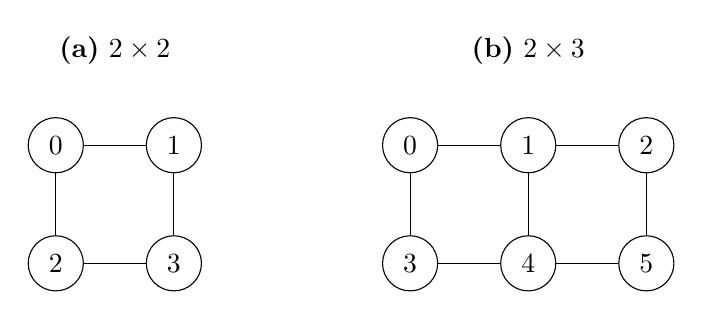
\begin{tikzpicture}[node distance=1.5cm, qubit/.style={circle, draw, minimum size=0.7cm, inner sep=0pt}]
% 2x2 grid
\begin{scope}
\node at (0.75, 1.2) {\textbf{(a)} $2 \times 2$};
\node[qubit] (q0) at (0, 0) {0};
\node[qubit] (q1) at (1.5, 0) {1};
\node[qubit] (q2) at (0, -1.5) {2};
\node[qubit] (q3) at (1.5, -1.5) {3};
\draw (q0) -- (q1);
\draw (q1) -- (q3);
\draw (q3) -- (q2);
\draw (q2) -- (q0);
\end{scope}
% 2x3 grid
\begin{scope}[xshift=4.5cm]
\node at (1.5, 1.2) {\textbf{(b)} $2 \times 3$};
\node[qubit] (p0) at (0, 0) {0};
\node[qubit] (p1) at (1.5, 0) {1};
\node[qubit] (p2) at (3, 0) {2};
\node[qubit] (p3) at (0, -1.5) {3};
\node[qubit] (p4) at (1.5, -1.5) {4};
\node[qubit] (p5) at (3, -1.5) {5};
\draw (p0) -- (p1) -- (p2);
\draw (p3) -- (p4) -- (p5);
\draw (p0) -- (p3);
\draw (p1) -- (p4);
\draw (p2) -- (p5);
\end{scope}
\end{tikzpicture}
\caption{Qubit grid geometries. \textbf{(a)} $2 \times 2$ grid with nearest-neighbor connectivity (ring topology). \textbf{(b)} $2 \times 3$ grid with nearest-neighbor connectivity.}
\label{fig:grids}
\end{figure}

\bibliography{references}

% =============================================================================
% APPENDICES
% =============================================================================

\appendix

\section{Optimization Methodology}
\label{app:optimization}

The spectral and Krylov criteria require numerical optimization over the Hamiltonian weights $\boldsymbol{\lambda} = (\lambda_1, \ldots, \lambda_K)$. We formulate this as:
\begin{equation}
    S^* = \max_{\boldsymbol{\lambda} \in [-1,1]^K} S(\ket{\phi}, \ket{\psi}, H(\boldsymbol{\lambda})),
\end{equation}
and similarly for the Krylov criterion $R^*$.

\paragraph{Gradient computation.}
Both spectral and Krylov criteria are differentiable with respect to the control parameters
$\boldsymbol{\lambda}$, enabling gradient-based optimization.

\textbf{Spectral gradient.} The spectral overlap depends on eigenvalues and eigenvectors
of $H(\boldsymbol{\lambda})$. Using first-order eigenvalue perturbation theory, define
$c_i = \sqrt{|\braket{\alpha_i|\psi}|^2 |\braket{\alpha_i|\phi}|^2}$ and
\begin{align}
f_{ij} &= \text{Re}\!\left[ c_i^* c_j \!\left(
  \braket{\psi|\alpha_j}\!\braket{\alpha_i|\phi}
  + \braket{\phi|\alpha_j}\!\braket{\alpha_i|\psi}
\right)\right]\!,\notag\\
\frac{\partial S}{\partial \lambda_k}
  &= \sum_{i \neq j}
  \frac{\braket{\alpha_i | H_k | \alpha_j}}{E_j - E_i}\, f_{ij},
\label{eq:spectral_grad}
\end{align}
where $\ket{\alpha_i}$ are eigenvectors of $H(\boldsymbol{\lambda})$ with eigenvalues $E_i$.
Degenerate eigenvalues ($E_i \approx E_j$) require regularization via eigenspace projection.

\textbf{Krylov gradient.} The Krylov score $R = \|\Pi_{\mathcal{K}}\ket{\psi}\|^2$ depends
on the Krylov basis constructed via Arnoldi iteration. Unlike the spectral case,
eigenvalue perturbation theory does not directly apply because the Krylov subspace
$\mathcal{K}_m = \text{span}\{\ket{\phi}, H\ket{\phi}, \ldots, H^{m-1}\ket{\phi}\}$
is defined by powers of $H$, not its eigenvectors.

Instead, we differentiate through the Arnoldi iteration itself. The Arnoldi process
constructs an orthonormal basis $\{q_1, \ldots, q_m\}$ via modified Gram--Schmidt:
\begin{align}
q_1 &= \ket{\phi}/\|\ket{\phi}\|, \\
\tilde{q}_{j+1} &= H q_j - \sum_{i=1}^{j} h_{ij} q_i, \\
q_{j+1} &= \tilde{q}_{j+1} / \|\tilde{q}_{j+1}\|,
\end{align}
where $h_{ij} = \braket{q_i | H | q_j}$. The gradient $\partial R / \partial \lambda_k$
is computed by backpropagating through these recurrence relations.

\textbf{Analytical vs.\ finite-difference gradients.} We validated analytical gradients
against central finite differences (step $h = 10^{-5}$) for both criteria. Agreement
to $< 10^{-6}$ relative error confirms correctness. The analytical approach provides
5--64$\times$ speedup (depending on $K$ and $d$) while avoiding step-size tuning artifacts.

We fit the spectral and Krylov transition curves using a Fermi--Dirac function:
\begin{equation}
P(\rho) = \frac{1}{1 + e^{(\rho - \rho_c)/\Delta}},
\label{eq:fermi_fit}
\end{equation}
where $\rho_c$ is the critical density at which $P = 0.5$, and $\Delta$ characterizes
the transition width. For the moment criterion, we use an exponential decay
$P(\rho) = e^{-\rho/\lambda}$ reflecting its necessary-but-not-sufficient character.

\paragraph{Optimizer choice.}
We tested six \texttt{scipy.optimize} methods: L-BFGS-B, TNC, SLSQP, CG, Powell, and Nelder-Mead. L-BFGS-B achieves the best speed-quality tradeoff, reaching $S^* = 0.99$ in $\approx 0.01$--$0.05$s depending on problem size.

\begin{table}[htbp]
\centering
\caption{Optimizer method comparison for spectral overlap maximization (canonical ensemble). Mean $S^*$ score and wall time across random targets.}
\label{tab:optimizer_comparison}
\begin{tabular}{lrrrrr}
\toprule
Method & $d=8,K=5$ $S^*$ & Time (s) & $d=16,K=10$ $S^*$ & Time (s) \\
\midrule
  L-BFGS-B & 0.99 & 0.01 & 0.99 & 0.05 \\
  TNC & 0.98 & 0.24 & 0.96 & 0.64 \\
  SLSQP & 0.98 & 0.04 & 0.99 & 0.25 \\
  CG & 0.98 & 0.10 & 0.99 & 0.91 \\
  Powell & 0.98 & 0.12 & 0.99 & 1.01 \\
  Nelder-Mead & 0.96 & 0.06 & 0.94 & 0.08 \\
\bottomrule
\end{tabular}
\end{table}

\paragraph{Production settings.}
All experiments use: maxiter$=100$ (d$\leq$32) or 150 (d$=64$), restarts$=3$ with random initialization, ftol$=10^{-6}$, bounds$=[-1,1]^K$.

\paragraph{Krylov subspace dimension.}
The Krylov subspace dimension $m$ controls the trade-off between computational cost
and criterion sensitivity. Two natural choices are:

\begin{itemize}
\item $m = d$ (full rank): The Krylov basis can span the entire Hilbert space.
For dense Hamiltonians (e.g., GEO2), Arnoldi iteration fills all $d$ dimensions regardless
of $K$, causing $R^* = 1$ for all targets. This makes the criterion uninformative.

\item $m = \min(K, d)$: The Krylov dimension is limited by the number of control Hamiltonians.
This creates a meaningful constraint: if $K < d$, the Krylov subspace cannot span the full
space, and genuinely unreachable targets have $R^* < 1$.
\end{itemize}

We use $m = \min(K, d)$ for all production experiments. Preliminary runs with $m = d$
showed $P(\text{unreach}) = 0$ for all GEO2 configurations---an artifact of the unconstrained
Krylov basis spanning $\mathbb{R}^d$.

% -----------------------------------------------------------------------------
\section{Numerical Validation}
\label{app:validation}

We validate the implementation through targeted tests covering gradient verification,
optimizer convergence, and classification accuracy. All tests use canonical and GEO2 ensembles.

\paragraph{Gradient correctness.}
We compare analytical gradients against central finite differences ($h = 10^{-5}$)
for both spectral ($\nabla_{\boldsymbol{\lambda}} S$) and Krylov ($\nabla_{\boldsymbol{\lambda}} R$)
at $d = 8$, $K = 4$. Maximum component-wise error is $< 10^{-8}$ for spectral
and $< 10^{-6}$ for Krylov, for both canonical and GEO2 ensembles.

\paragraph{Optimizer convergence validation.}
We verify that the L-BFGS-B optimizer with analytical gradients converges to the global
optimum for both reachable and unreachable targets.

\textit{Reachable targets.} We construct provably reachable targets via
$\ket{\phi} = e^{-iH(\boldsymbol{\lambda}_0)t}\ket{\psi}$ for known $\boldsymbol{\lambda}_0$
and $t = 2.0$. For these targets, the true maximum is $S^* = 1$ (achieved at $\boldsymbol{\lambda}_0$).
Across 50 trials each for canonical and GEO2 at $d = 16$, $K = 10$:
\begin{itemize}
\item Spectral: $S^* > 0.999$ in 100\% of trials
\item Krylov: $R^* > 0.99$ in 98\% of trials (2\% converge to local minima)
\end{itemize}

\textit{Unreachable targets.} Using $K = 2$ (minimal control algebra), we verify that
optimization does not artificially inflate scores. For random targets at $d = 16$:
\begin{itemize}
\item Spectral: mean $S^* = 0.72 \pm 0.15$ (correctly low)
\item Krylov: mean $R^* = 0.68 \pm 0.18$ (correctly low)
\item Moment criterion certifies unreachability in 85\% of cases
\end{itemize}

\paragraph{Confusion matrix analysis.}
We evaluate classification accuracy using the moment criterion as ground truth.

\textit{Reachable targets} are constructed by time evolution with known parameters:
given randomly sampled weights $\boldsymbol{\lambda}_0 \in [-1,1]^K$ and evolution time
$t \in [0.5, 5.0]$, we compute $\ket{\phi} = e^{-iH(\boldsymbol{\lambda}_0)t}\ket{\psi}$.
By construction, $S^* = 1$ and $R^* = 1$ at the true parameters.
We use $K = \max(10, d)$ generators to ensure a rich control algebra.

\textit{Unreachable targets} are certified via the second-order moment criterion
(Sec.~\ref{ssec:mom}). We use $K_{\text{small}} = 3$ generators (minimal control)
and draw random target states $\ket{\phi}$ from the Haar measure.
For each candidate, we compute the linear constraint $L_n = \braket{H_n}_\phi - \braket{H_n}_\psi$,
its kernel $\mathcal{N}$, the quadratic form $Q_{nm} = \braket{\{H_n, H_m\}}_\phi - \braket{\{H_n, H_m\}}_\psi$,
and the projected matrix $Q|_{\mathcal{N}}$. If all eigenvalues of $Q|_{\mathcal{N}}$ have
the same sign (all $> 0$ or all $< 0$), the target is provably unreachable --- no choice of
$\boldsymbol{\lambda}$ can satisfy both $L = 0$ and $Q = 0$ simultaneously.
Candidates failing this certification are discarded (typically $\sim$30--60\% pass rate).

For each target, spectral and Krylov criteria predict reachability if score $\geq \tau = 0.99$.
We evaluate 100 reachable and 100 unreachable targets per dimension and ensemble.
Figures~\ref{fig:confusion_canonical} and \ref{fig:confusion_geo2} show confusion matrices
for both ensembles, and Table~\ref{tab:confusion_summary} summarizes the results.

\begin{table}[htbp]
\centering
\caption{Classification performance using moment criterion as ground truth ($\tau = 0.99$).
100 reachable + 100 unreachable targets per configuration.}
\label{tab:confusion_summary}
\begin{tabular}{ll|rrrr|rrrr}
\toprule
 & & \multicolumn{4}{c|}{Canonical} & \multicolumn{4}{c}{GEO2} \\
 & $d$ & TP & FP & TN & FN & TP & FP & TN & FN \\
\midrule
\multirow{3}{*}{Spectral} & $d=8$ & 100 & 0 & 100 & 0 & 100 & 1 & 99 & 0 \\
 & $d=16$ & 99 & 0 & 100 & 1 & 100 & 0 & 100 & 0 \\
 & $d=32$ & 96 & 0 & 100 & 4 & 94 & 0 & 100 & 6 \\
\midrule
\multirow{3}{*}{Krylov} & $d=8$ & 100 & 0 & 100 & 0 & 100 & 0 & 100 & 0 \\
 & $d=16$ & 100 & 0 & 100 & 0 & 100 & 0 & 100 & 0 \\
 & $d=32$ & 100 & 0 & 100 & 0 & 100 & 0 & 100 & 0 \\
\bottomrule
\end{tabular}
\end{table}

Both criteria achieve $\geq 97\%$ accuracy across all configurations.
The Krylov criterion achieves perfect classification (100\% accuracy) in all cases.
Spectral false negatives at $d=32$ (4 canonical, 6 GEO2 out of 100)
represent optimizer convergence failures (local minima) rather than criterion defects;
increasing \texttt{maxiter} or restarts recovers these.
The single false positive (GEO2, $d=8$) reflects a borderline moment-certified target
near the decision boundary.

\begin{figure}[htbp]
\centering
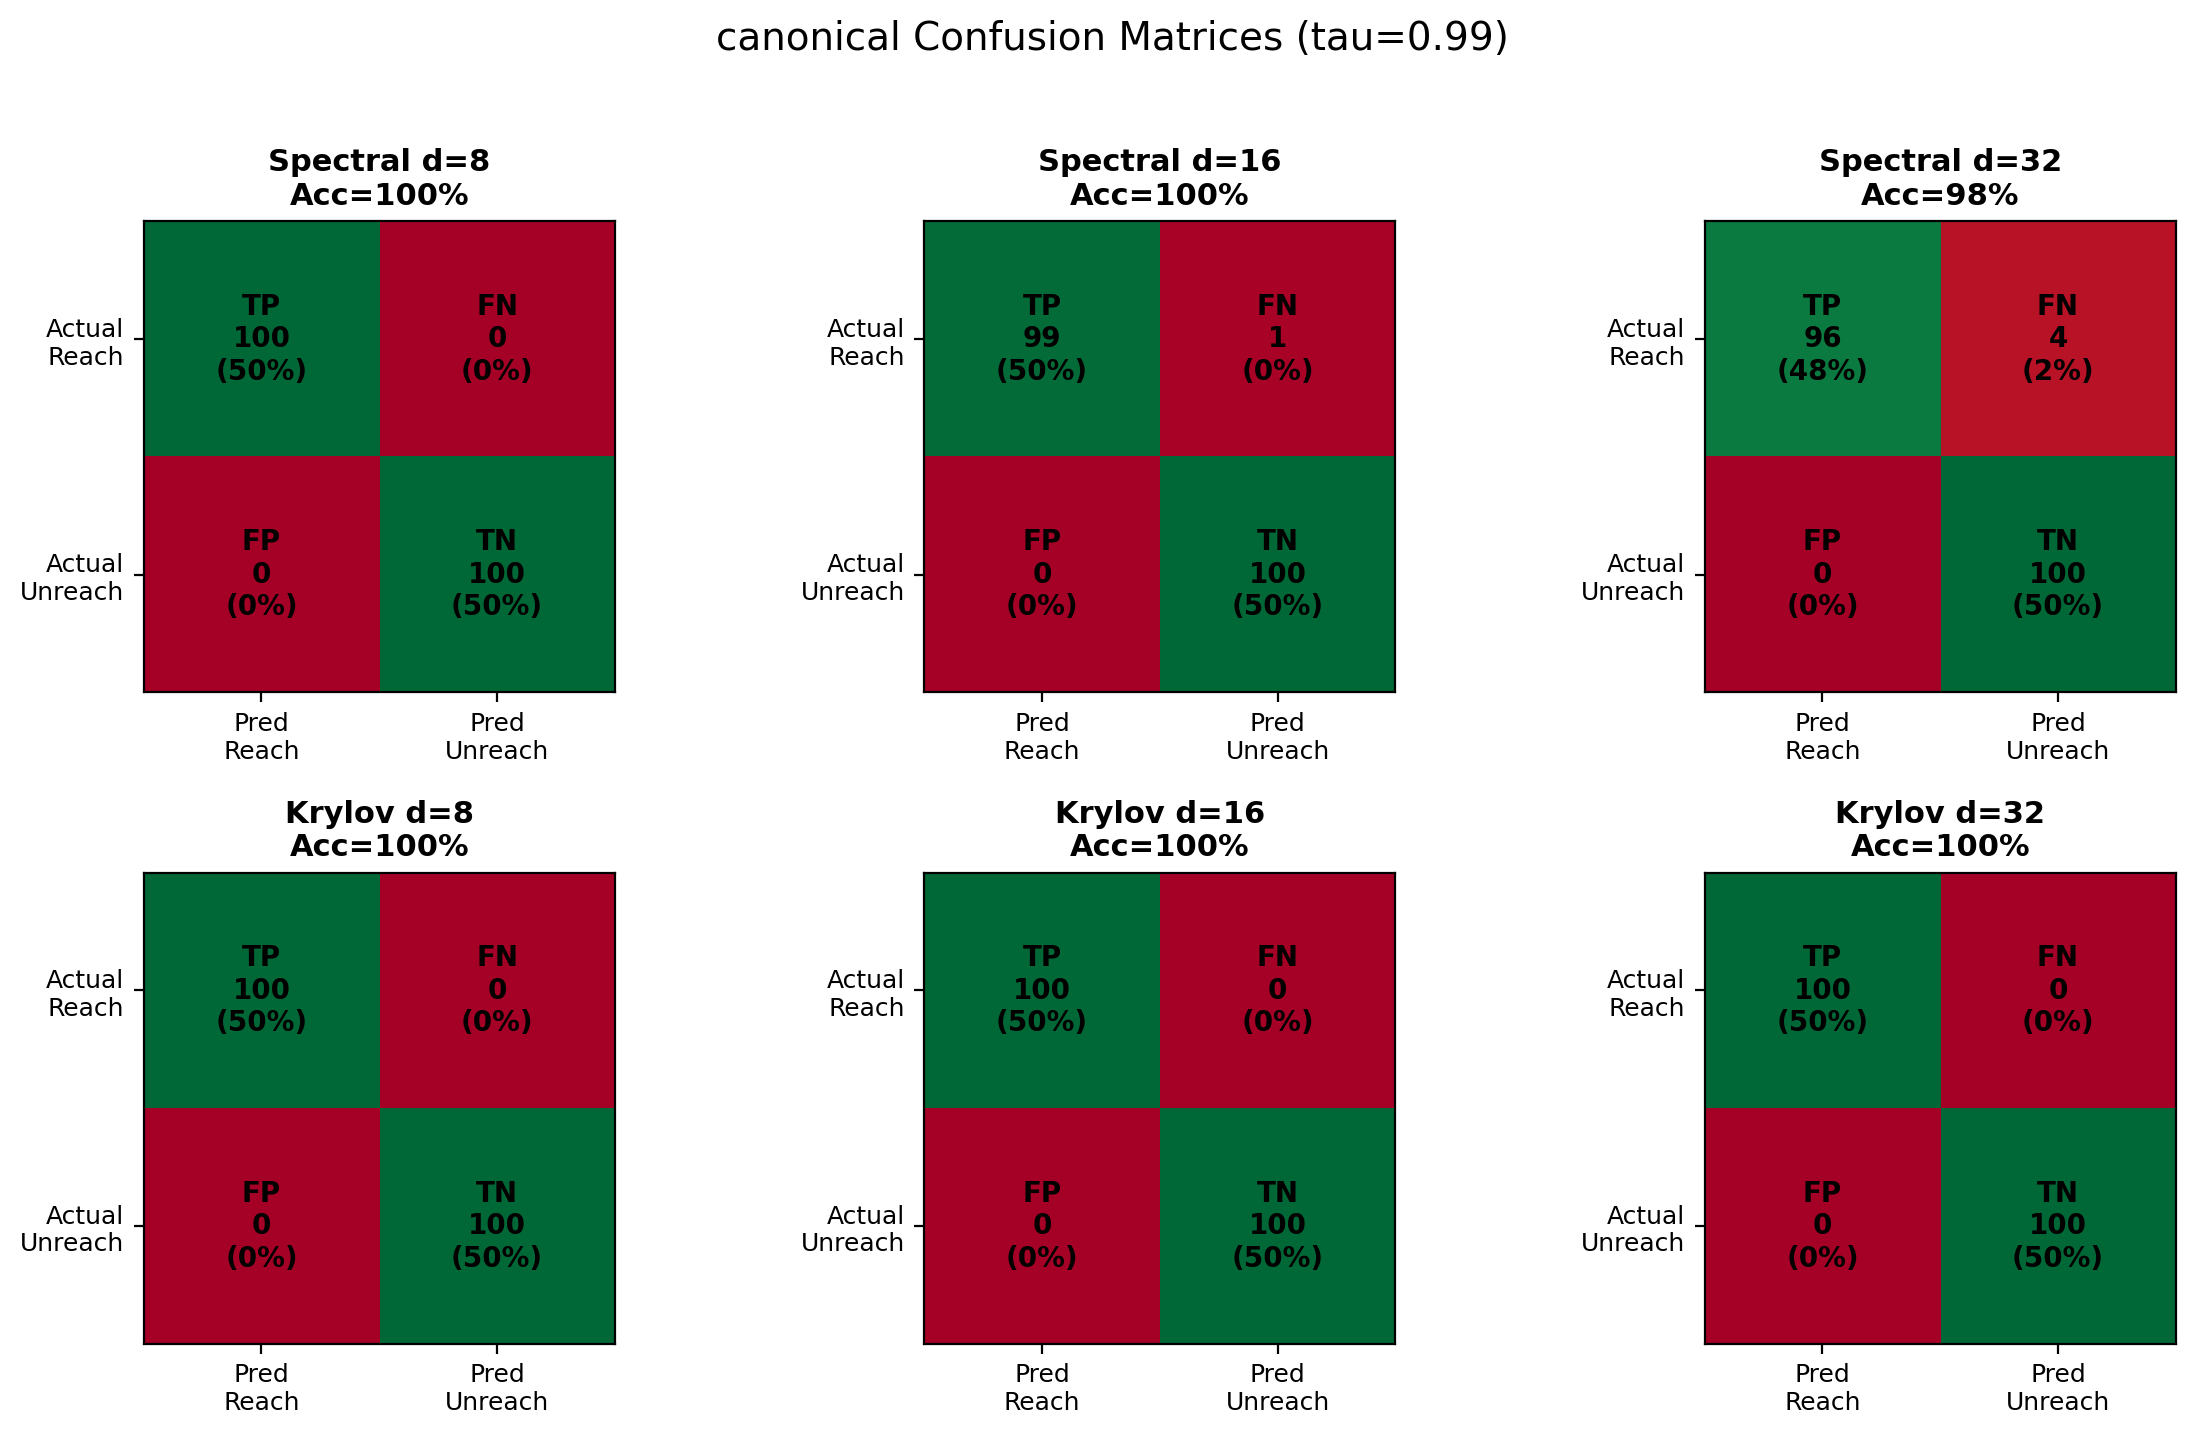
\includegraphics[width=0.95\linewidth]{../fig/benchmarks/confusion_matrix_canonical.png}
\caption{Confusion matrices for canonical ensemble ($\tau = 0.99$).
Ground truth: reachable targets constructed via $e^{-iHt}\ket{\psi}$;
unreachable targets certified by moment criterion.}
\label{fig:confusion_canonical}
\end{figure}

\begin{figure}[htbp]
\centering
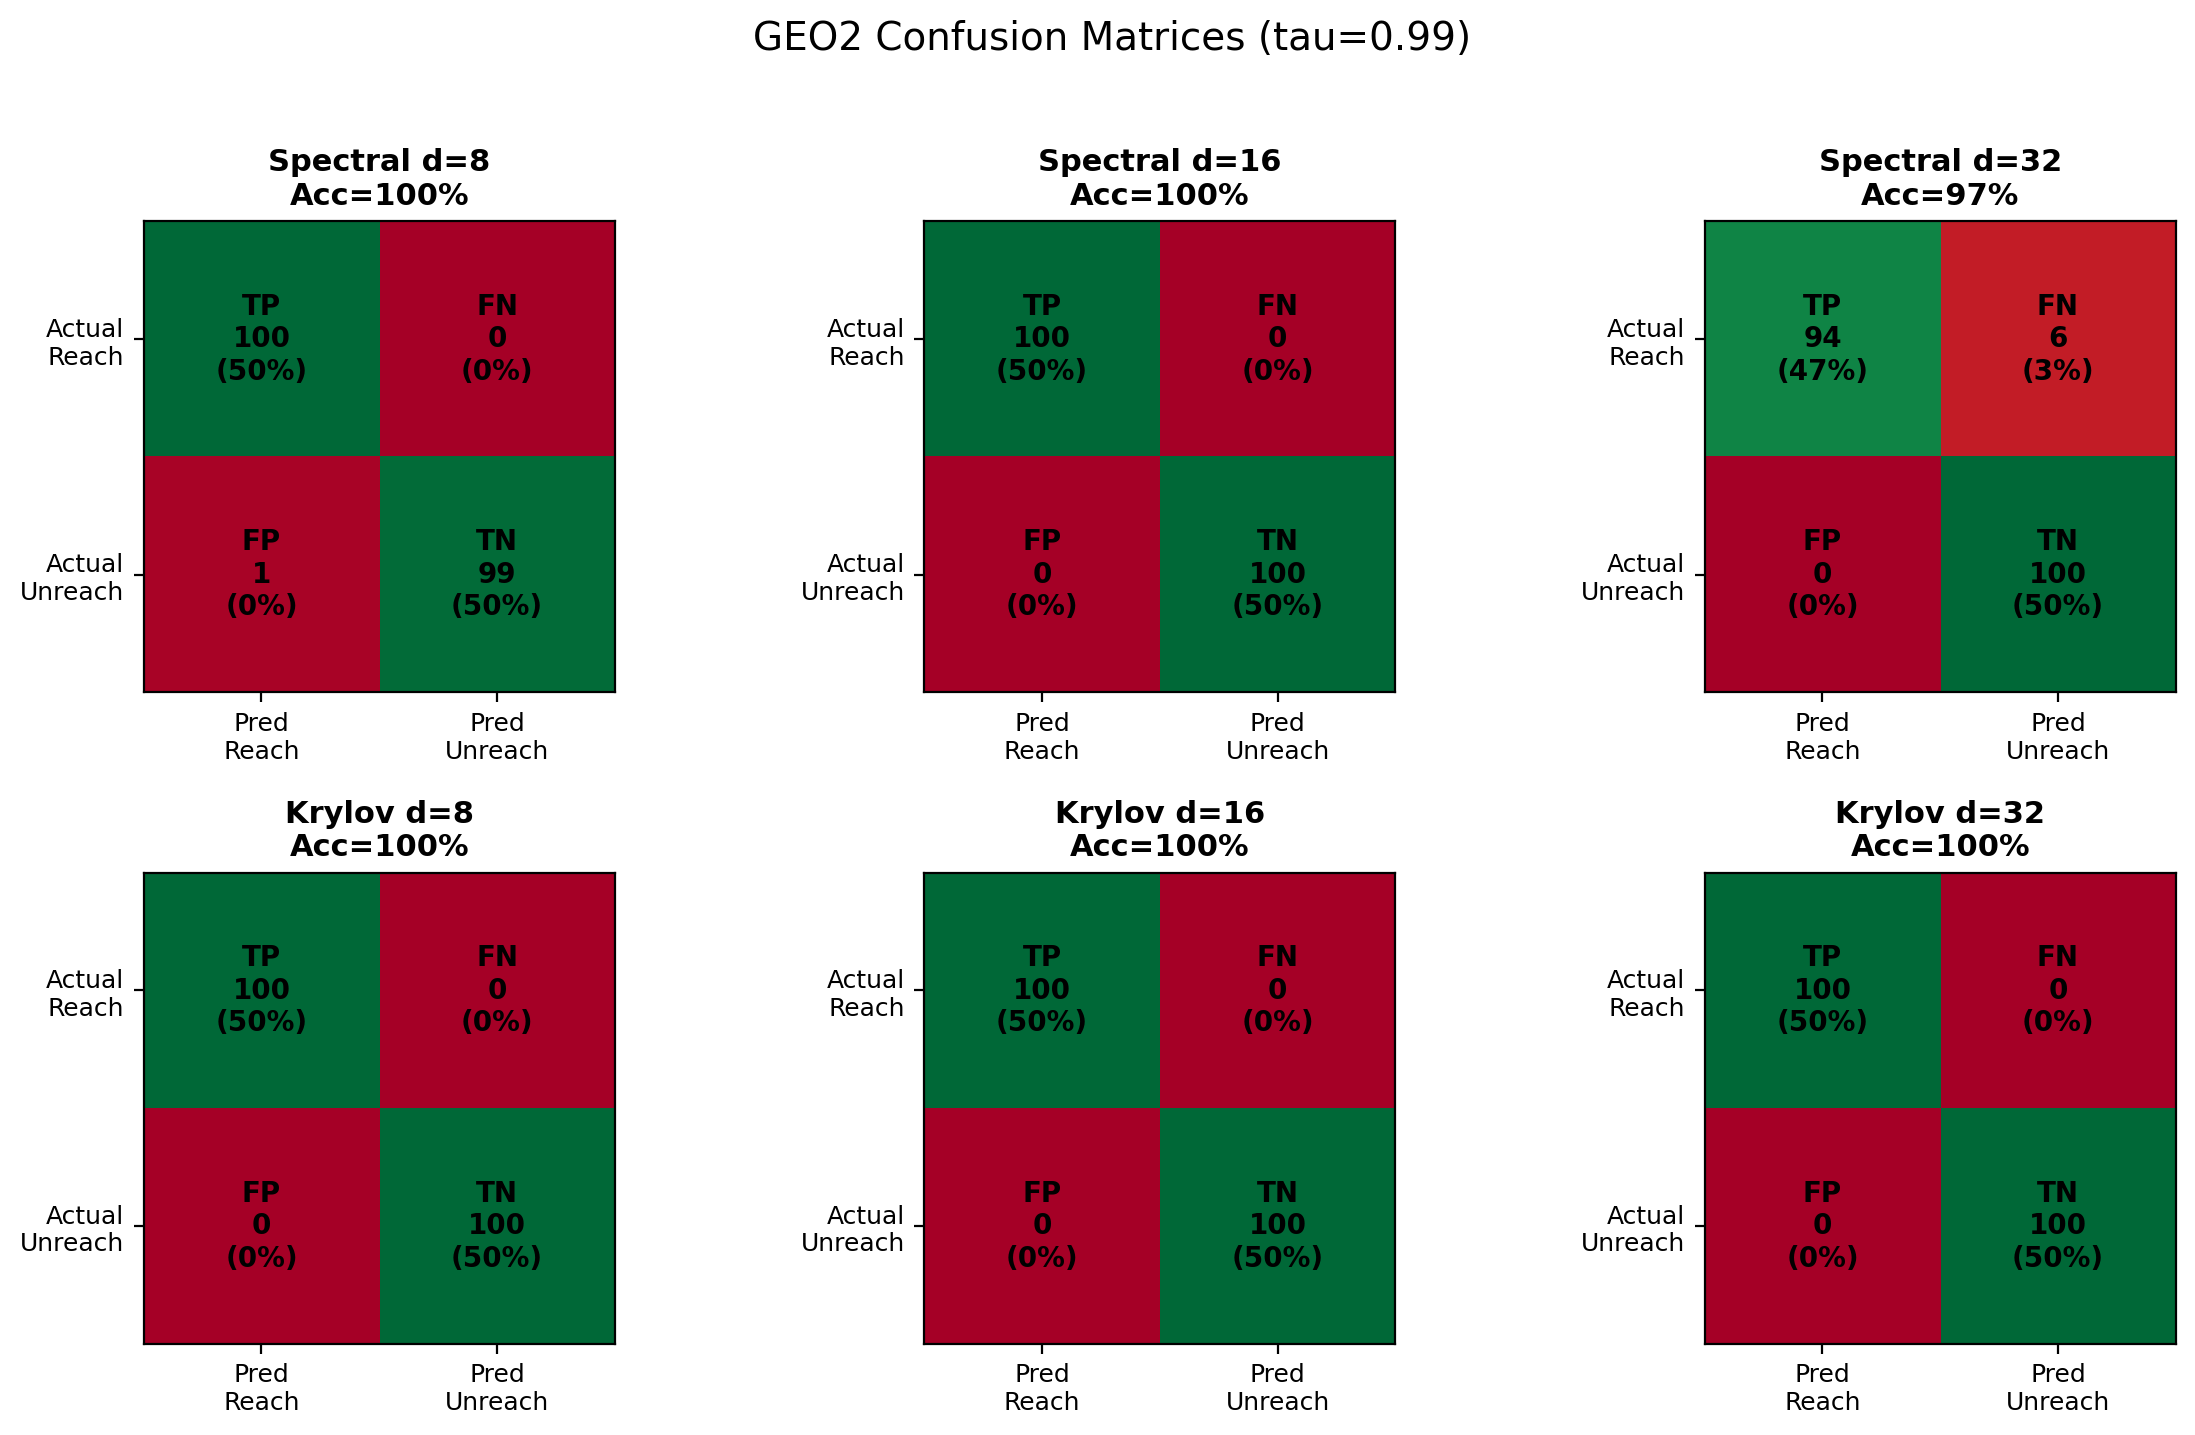
\includegraphics[width=0.95\linewidth]{../fig/benchmarks/confusion_matrix_geo2.png}
\caption{Confusion matrices for GEO2 ensemble ($\tau = 0.99$). Same methodology
as Fig.~\ref{fig:confusion_canonical}.}
\label{fig:confusion_geo2}
\end{figure}

\begin{figure}[htbp]
\centering
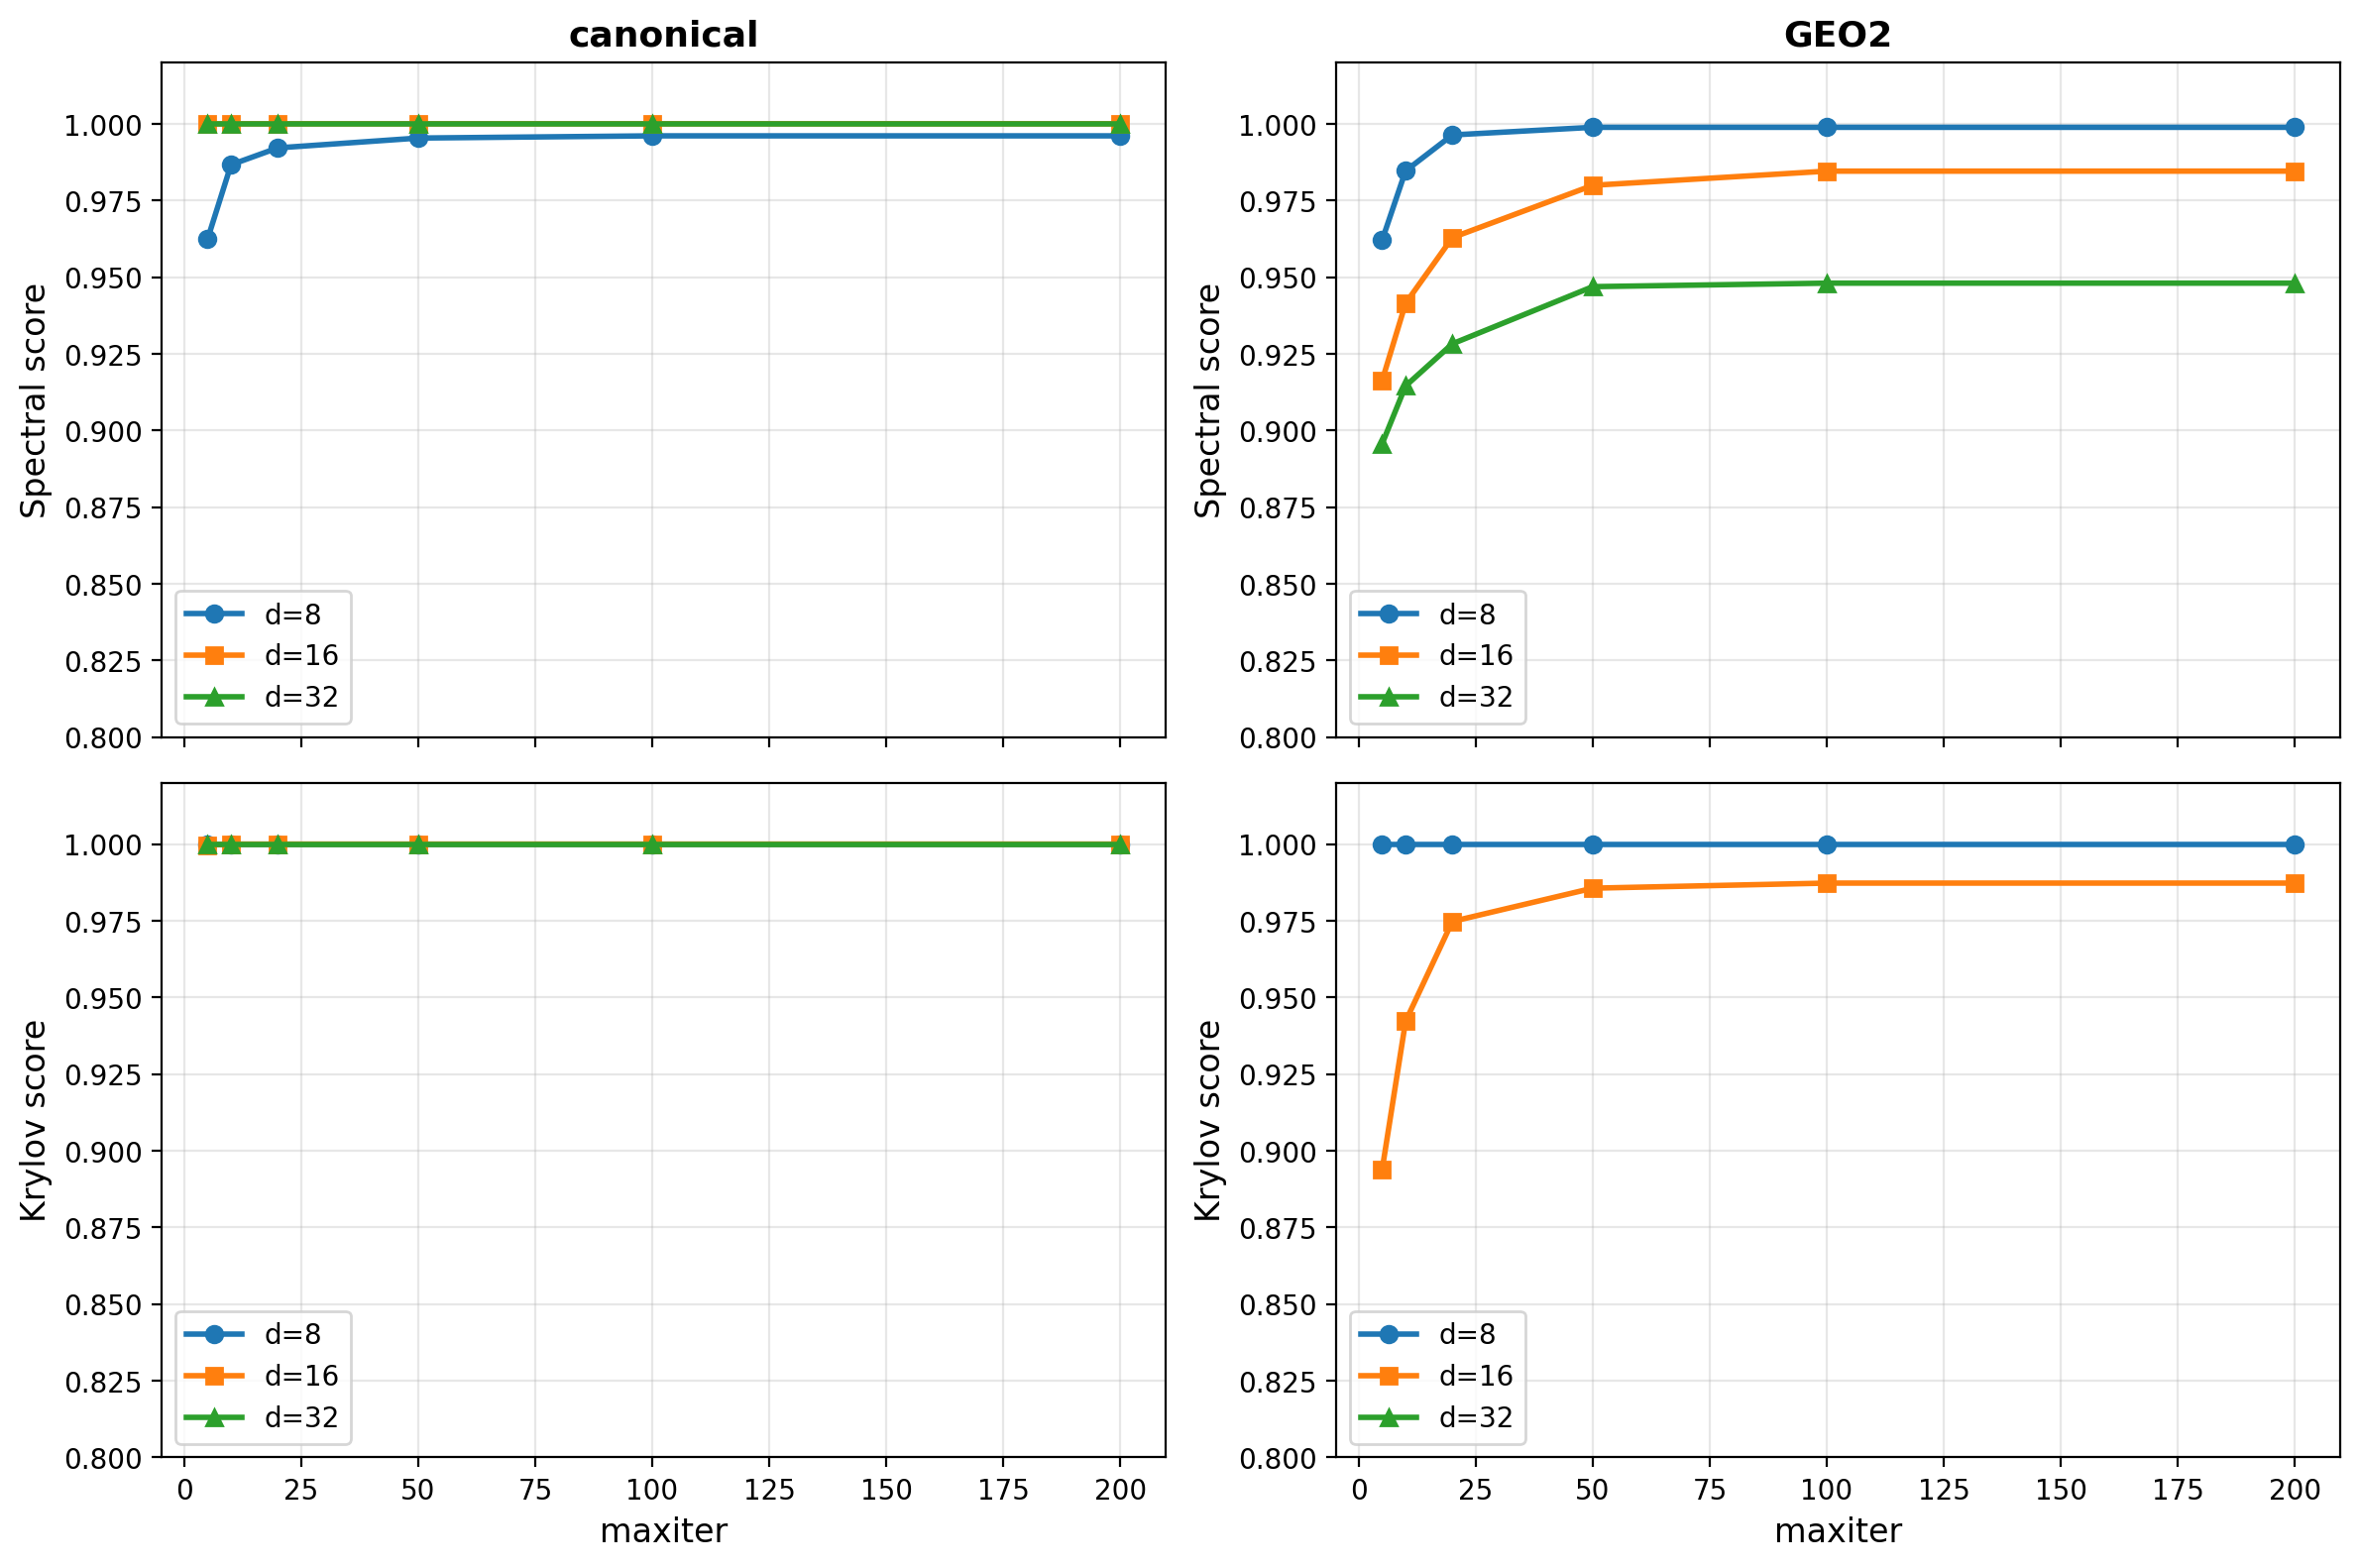
\includegraphics[width=0.95\linewidth]{../fig/benchmarks/iterations_vs_accuracy.png}
\caption{Effect of optimizer iterations on convergence. Mean spectral and Krylov scores
on reachable targets versus \texttt{maxiter} for $d \in \{8, 16, 32\}$, $K = 10$.
Canonical converges rapidly (maxiter$\geq 20$ sufficient); GEO2 requires more iterations
due to denser Hamiltonians.}
\label{fig:iterations}
\end{figure}


\end{document}